\chapter{The LHC and the CMS Detector} \label{chap-detector}

\section{The Large Hadron Collider} \label{sec-TheLargeHadronCollider}

The Large HAdron Collider (LHC) is currently the largest, and highest energy, particle accelerator ever created. Located, on average, one hundred metres under the Franco-Swiss border at Geneva, the LHC is installed in the 26.7 km tunnel that once contained the Large Electron-Positron Collider (LEP), and ran from 1989 until the end of 2000. The project was approved by the CERN council in December of 1994. Originally, the accelerator was designed as a two-stage project: constructed to run at a centre-of-mass energy of $\sqrt{s}=7$ TeV, and later an upgrade to $\sqrt{s}=14$ TeV. This was due to budget constraints which did not include contributions from non member states. 

After many setbacks, the first run began in 2010 and continued until the end of 2011 when the beam energy was then increased to $\sqrt{s}=8$ TeV for the whole of 2012 before shifting to Long Shutdown 1 (LS1) from 2013 to 2015. During LS1 the CERN accelerator complex, shown in Figure \ref{fig-CERNAcceleratorComplex}, was completely upgraded in order to run at a new unprecedented centre-of-mass energy of $\sqrt{s}=13$ TeV before ramping up to the original design energy of $\sqrt{s}=14$ TeV. 

\begin{figure}\label{fig-CERNAcceleratorComplex}
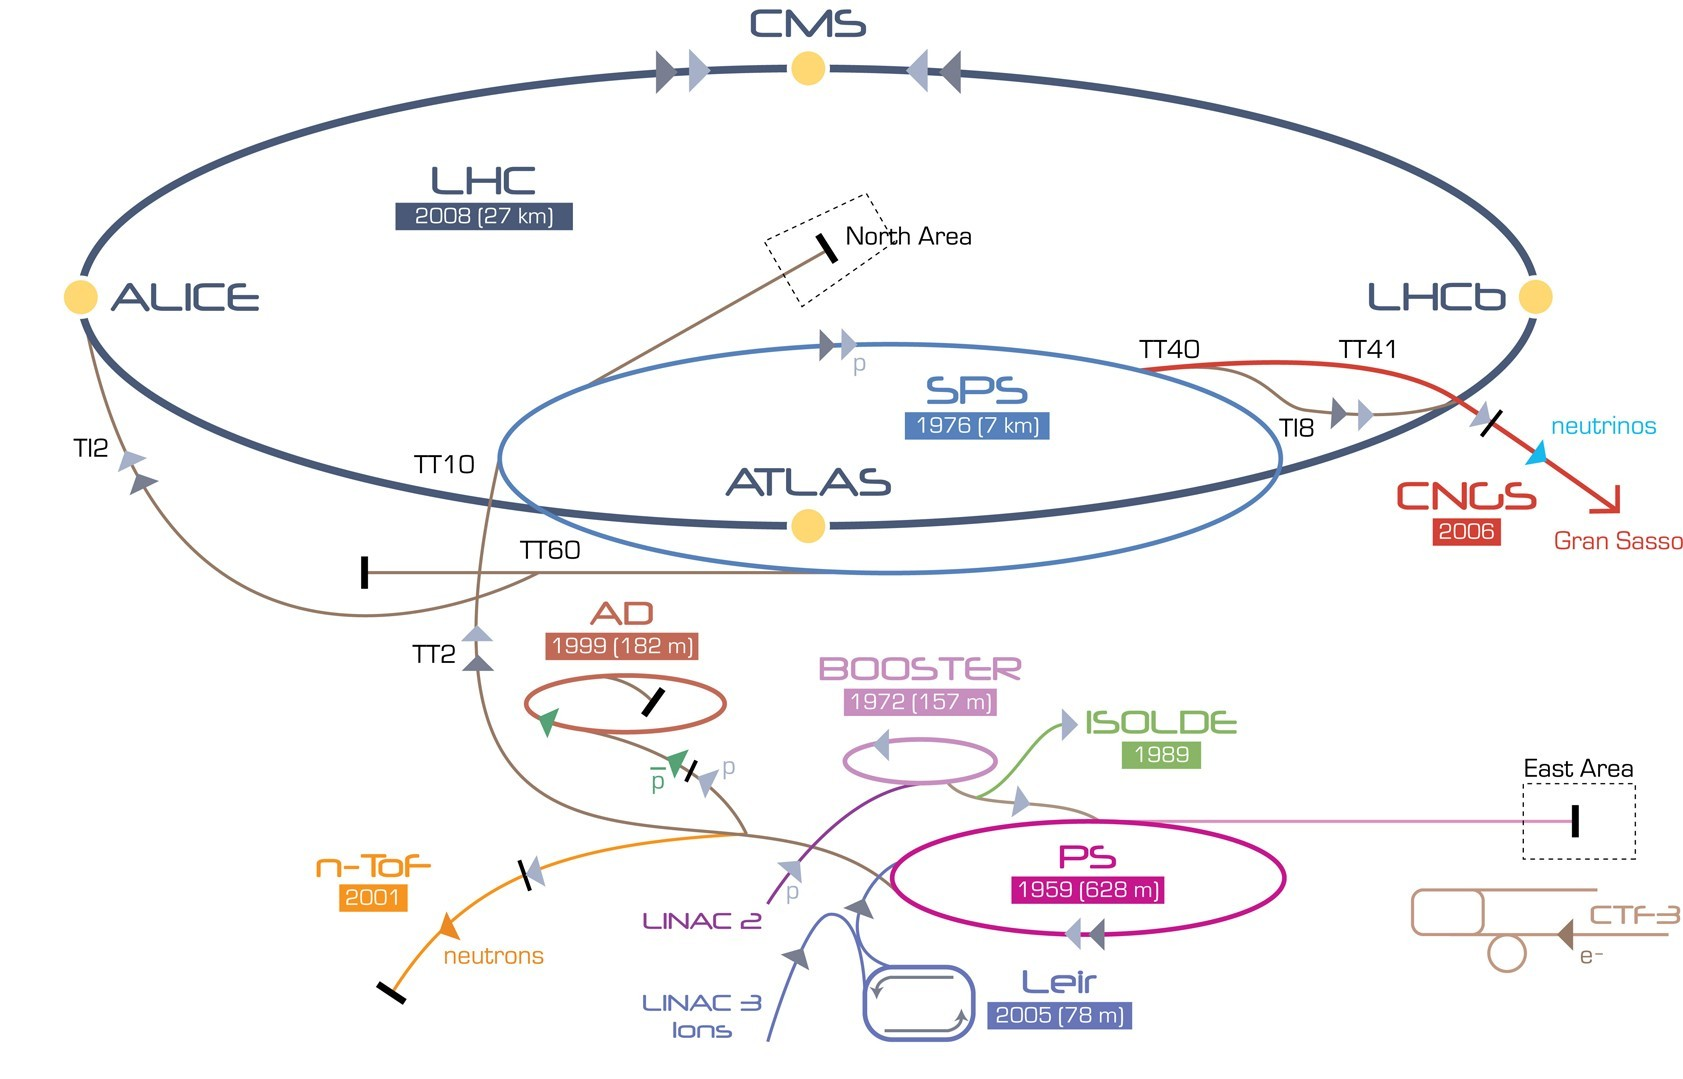
\includegraphics[width=\textwidth]{Figures/CERNAcceleratorComplex.jpg}
\caption{A full schematic of the full CERN accelerator complex \cite{}.}
\end{figure}

\subsection{Pre-LHC accelerator complex}

\subsection{Design of the LHC}

\begin{table} \label{tab-LHCparameters}
\begin{center}
\begin{tablular}{|c|c|}
\hline
	\multicolumn{2}{|c|}{\textbf{LHC Parameters}} \\
\hline
	tits & tits \\
\hline
\end{tabular}
\end{center}
\caption{LHC design parameters.}
\end{table}


\subsection{Physics goals}

\section{The CMS Detector} \label{sec-TheCMSDetector}

\begin{figure}\label{fig-CMSDetector}
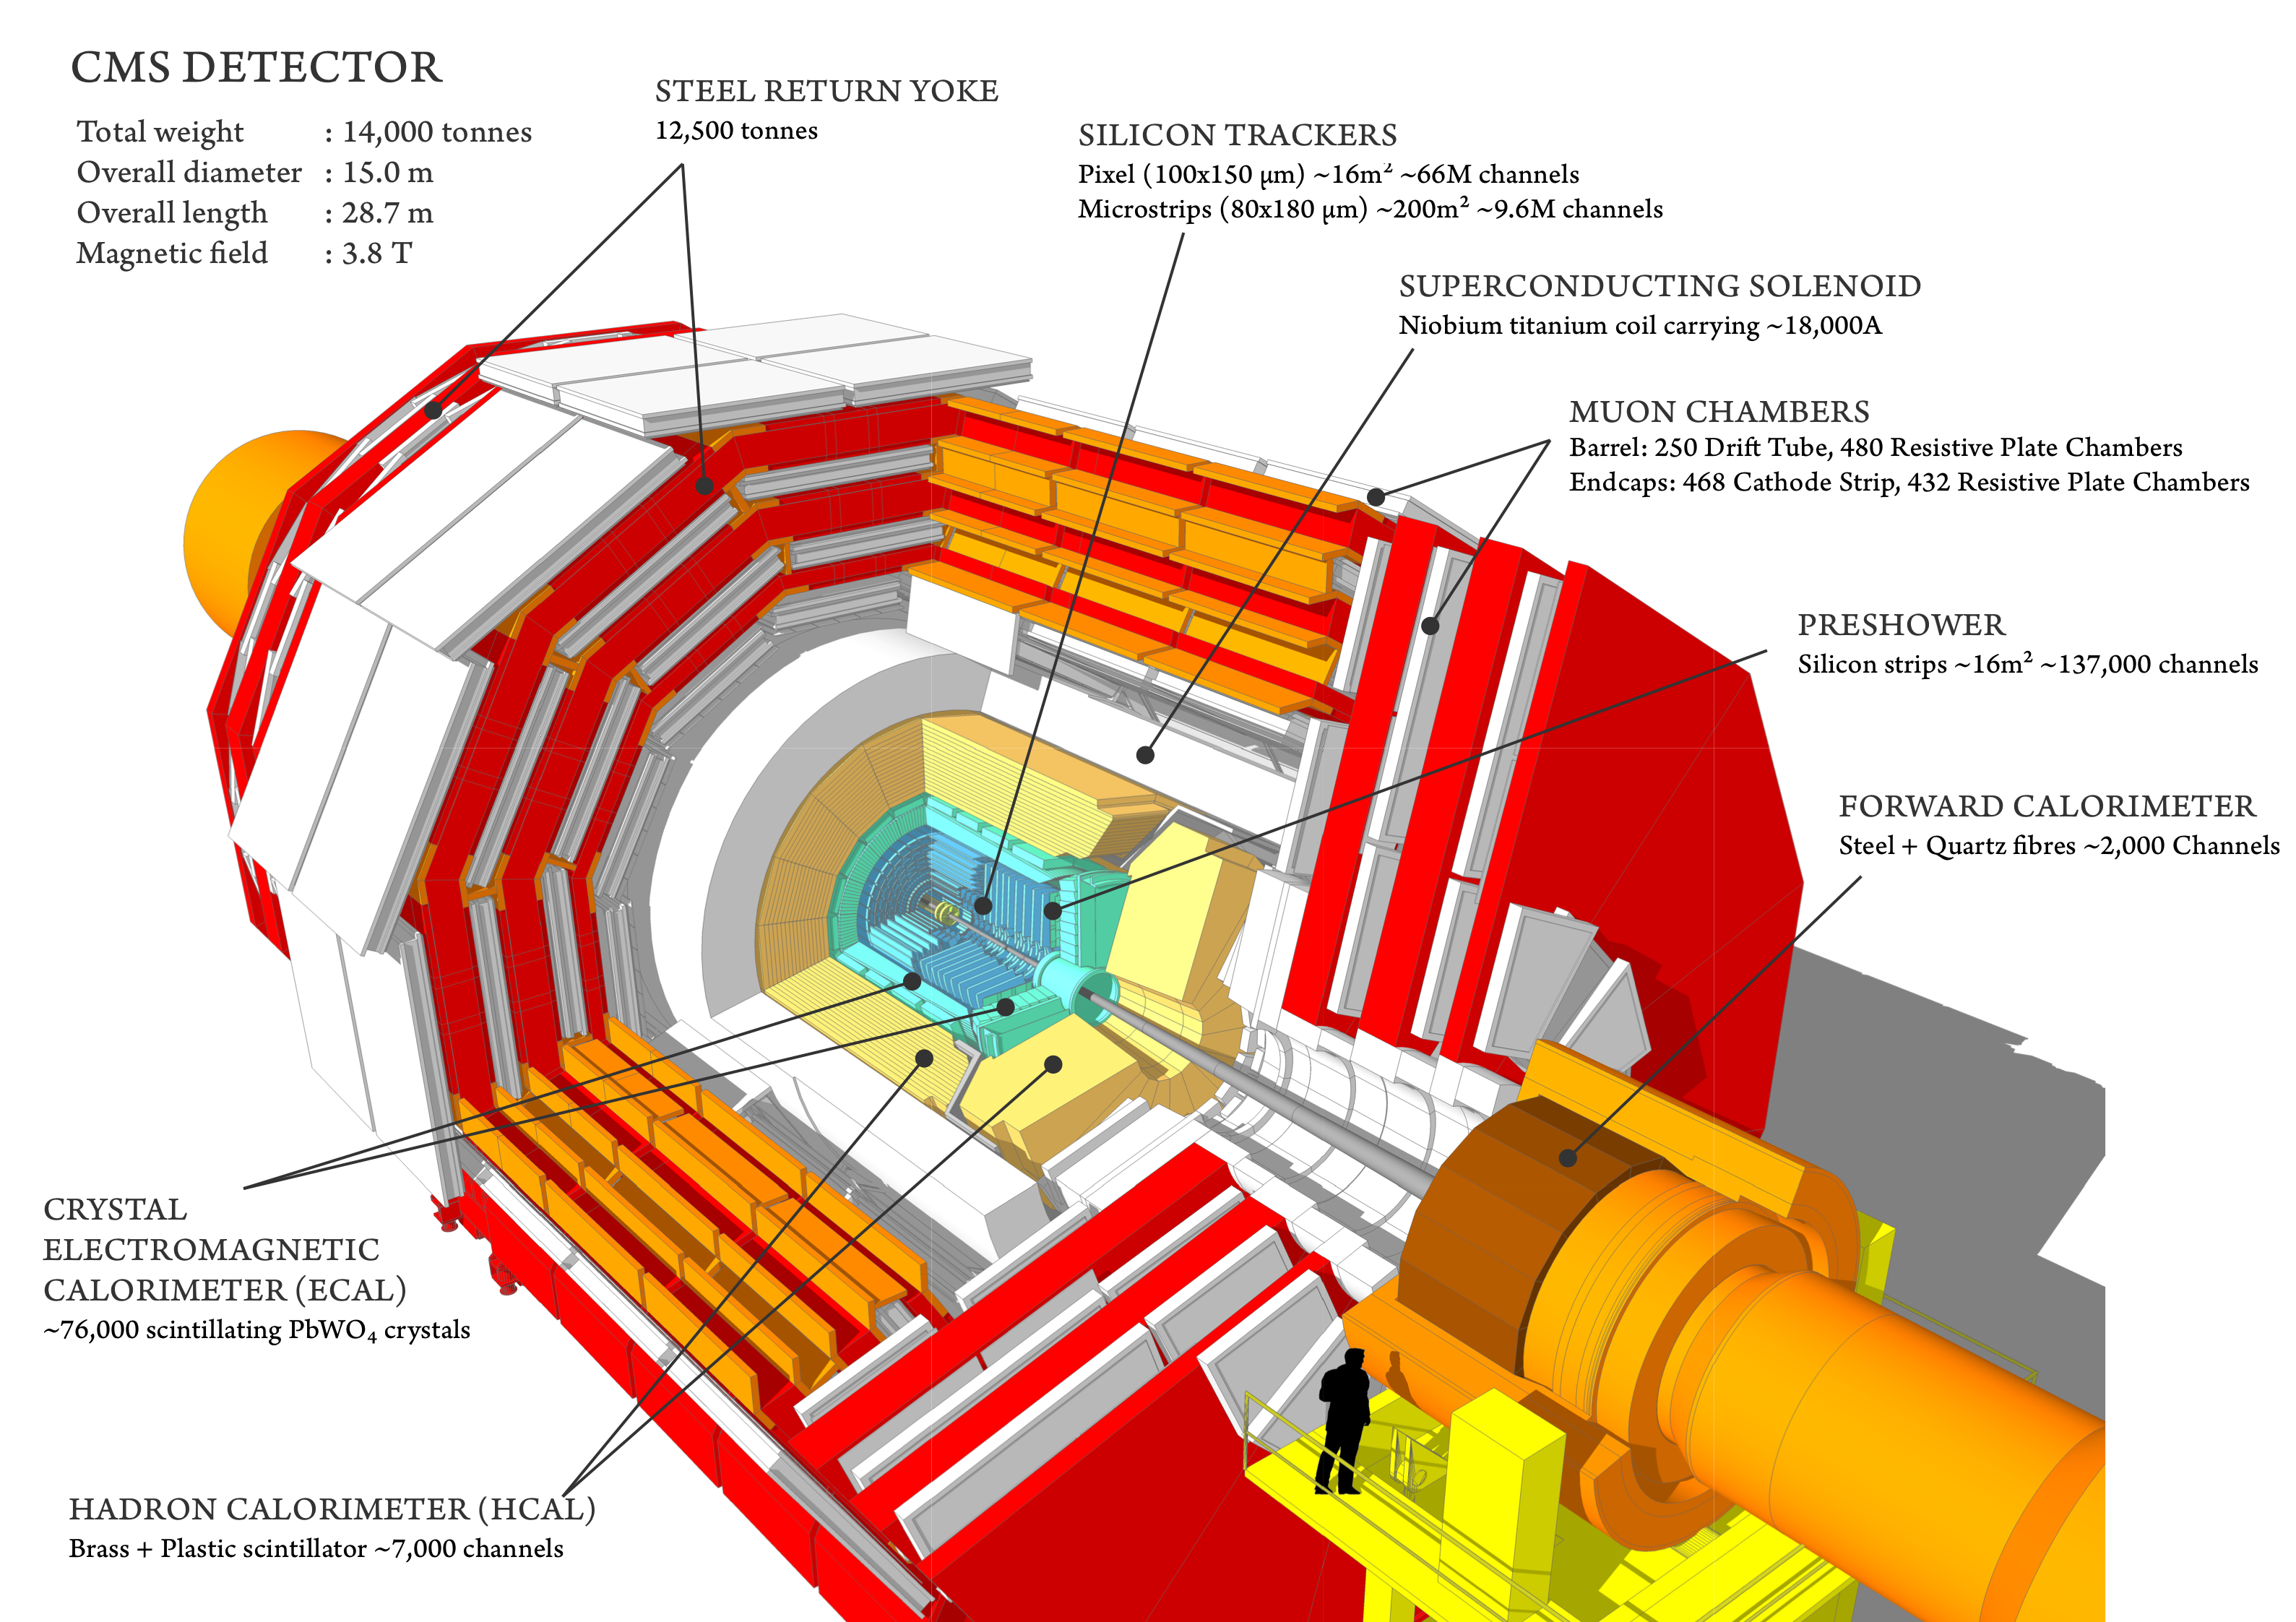
\includegraphics[width=\textwidth]{Figures/CMSDetector.png}
\caption{A cross-sectional view of the CMS detector \cite{}.}
\end{figure}

\section{Tracking System} \label{sec-TrackingSystem}

Figure \ref{fig-Tracker} schematic cross section through the CMS tracker. Each line represents a detector module. Double lines indicate back-to-back modules which deliver stereo hits \cite{CMSexperiment}.

\begin{figure}\label{fig-Tracker}
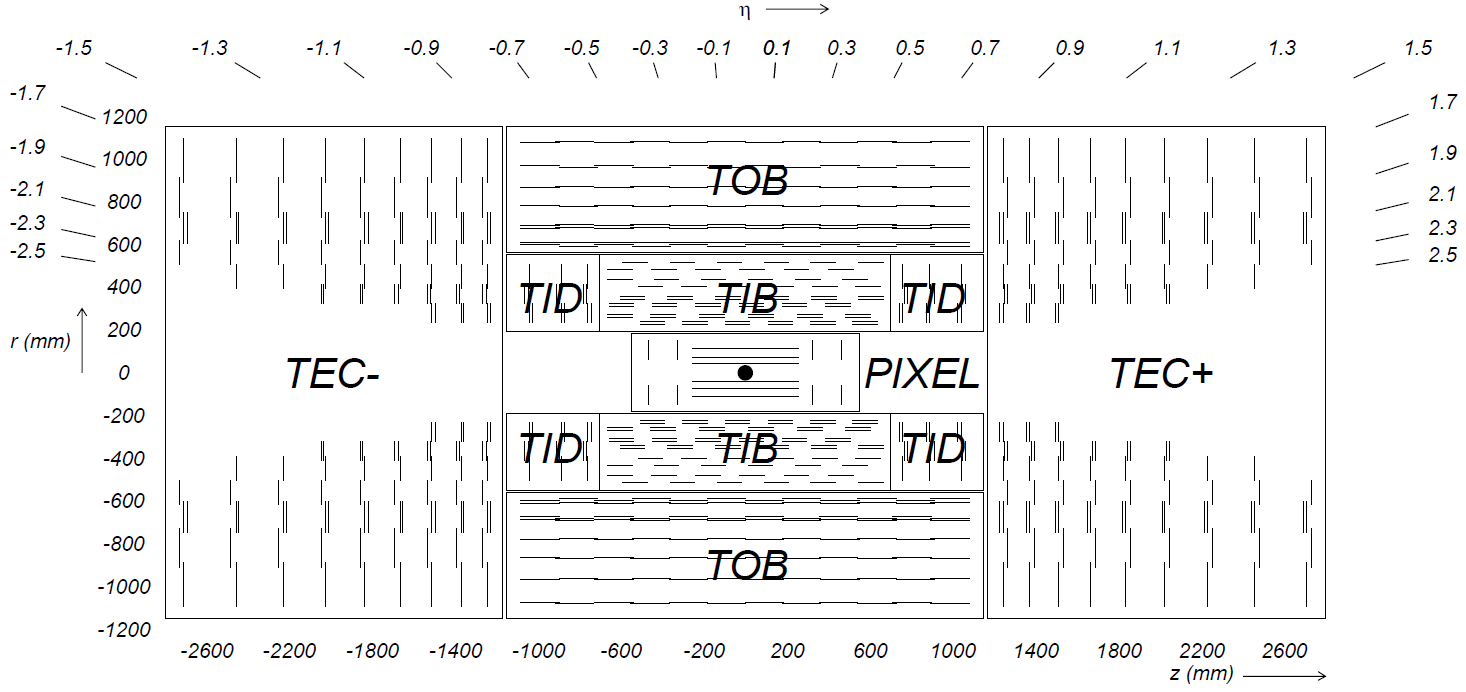
\includegraphics[width=\textwidth]{Figures/Tracker.png}
\caption{The subdetectors of the CMS silicon tracker system: TOB=outer barrel, TIB=inner barrel, TID=inner disc, TEC=endcaps, PIXEL=pixeldetector \cite{}.}
\end{figure}

\section{Electromagnetic Calorimeter} \label{sec-ElectromagneticCalorimeter}

\begin{figure}\label{fig-ECAL}
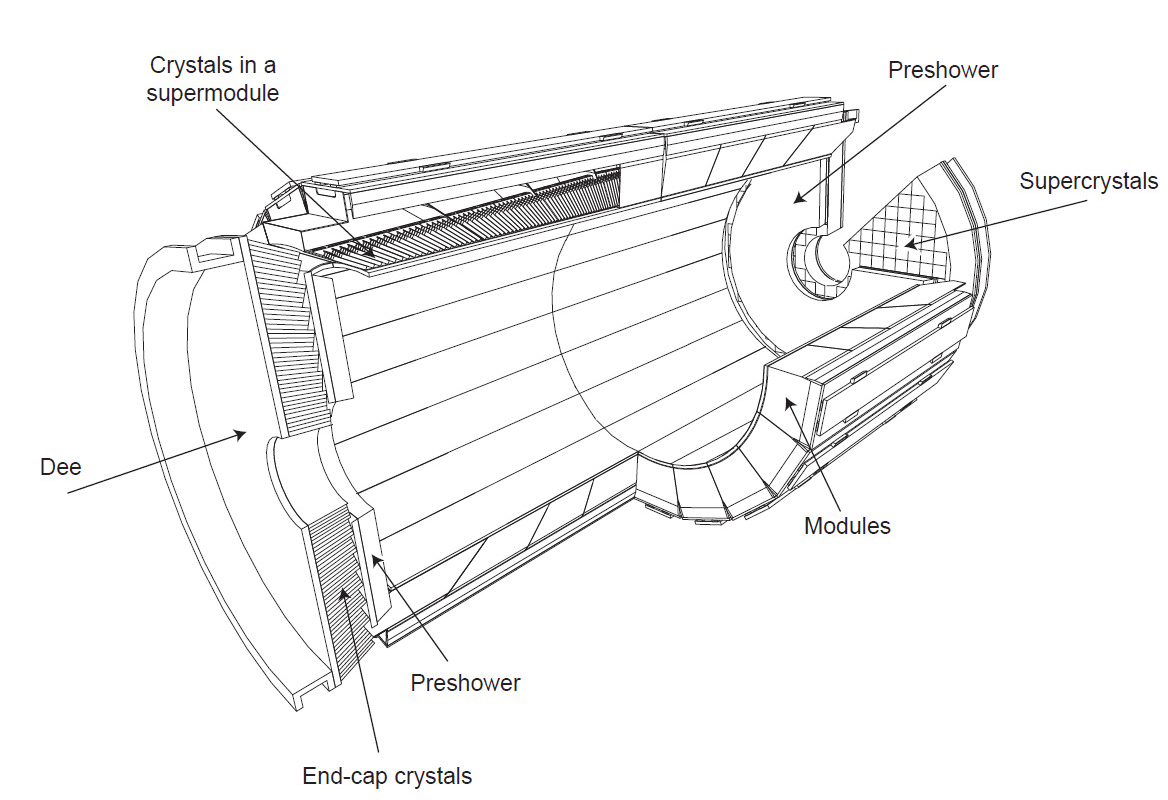
\includegraphics[width=\textwidth]{Figures/ECAL.png}
\caption{Geometric view of one quarter of the ECAL (top). Layout of the CMS electromagnetic calorimeter presenting the arrangement of crystal modules, supermodules, endcaps and the preshower in front (bottom) \cite{CMSexperiment}.}
\end{figure}

\begin{figure}\label{fig-ECALRapidity}
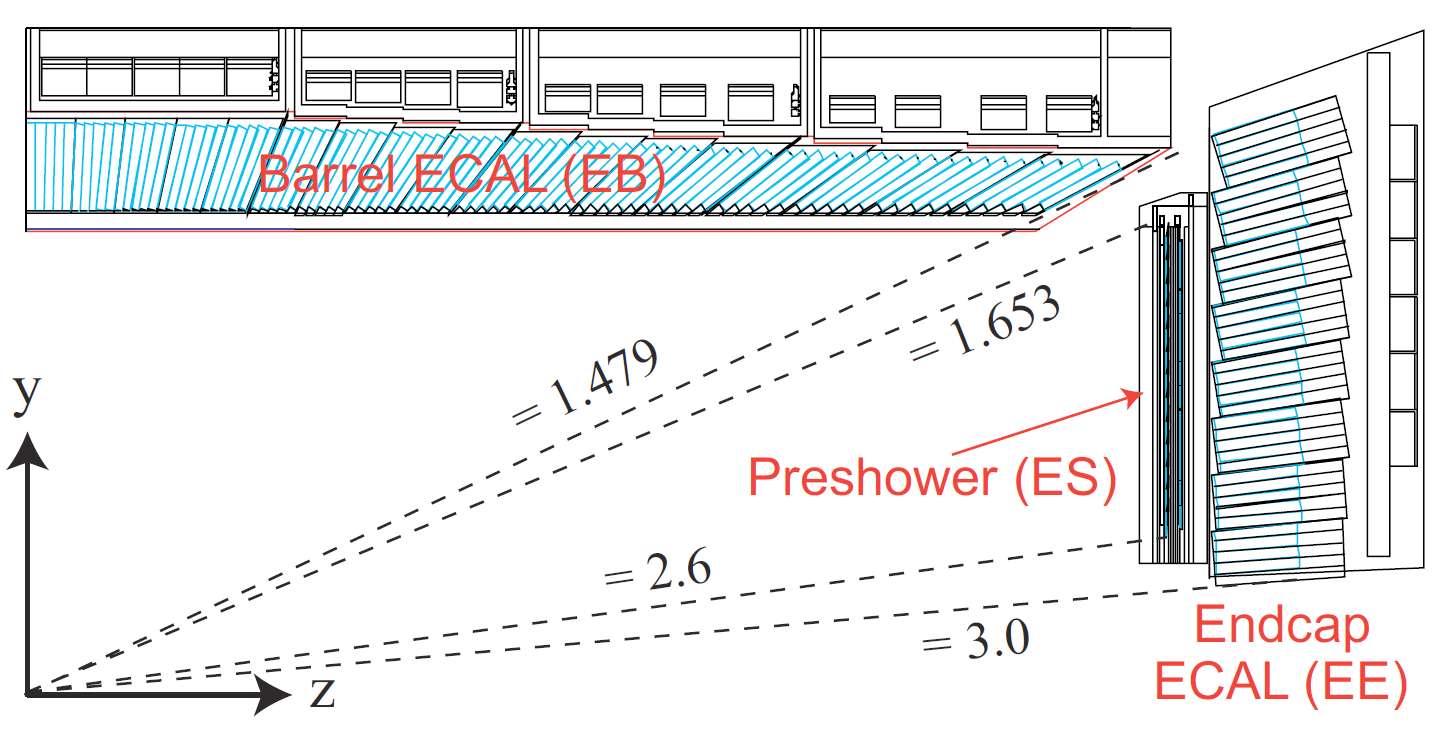
\includegraphics[width=\textwidth]{Figures/ECALRapidity.png}
\caption{Geometric view of one quarter of the ECAL (top). Layout of the CMS electromagnetic calorimeter presenting the arrangement of crystal modules, supermodules, endcaps and the preshower in front (bottom) \cite{CMSexperiment}.}
\end{figure}

\section{Hadron Calorimeter} \label{sec-HadronCalorimeter}

\section{Superconducting Solenoid} \label{sec-SuperconductingSolenoid}

\section{Muon System} \label{sec-MuonSystem}

\begin{figure}\label{fig-CMSLongitudinalView}
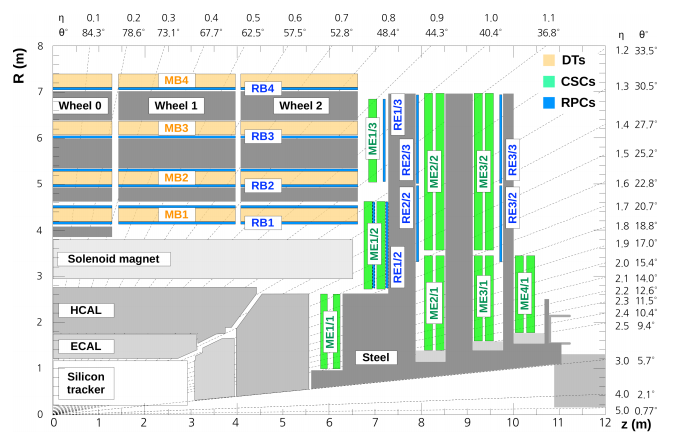
\includegraphics[width=\textwidth]{Figures/CMSLongitudinalView.png}
\caption{Layout of one quadrant of CMS. The figure shows the four DT stations in the barrel (MB1-MB4, yellow), the four CSC stations in the endcap (ME1-ME4, green), and the RPC stations (RB1-RB4 and RE1-RE3) \cite{CMSexperiment}.}
\end{figure}

\section{Trigger} \label{sec-Trigger}

\section{Particle Reconstruction} \label{sec-ParticleReconstruction}

\subsection{Electron identification}

\subsection{Muon reconstruction}

\subsection{Jet reconstruction}

\subsubsection{Jet energy corrections}

\subsubsection{Particle flow jet identification}

\section{Computing}

\subsection{Event Data Model}

\subsection{Analysis Software}

\section{Monte Carlo Simulation}

\begin{sidewaystable}
\begin{center}

\begin{tabular}{|l| p{12.5cm} |c|p{2cm}|}
\hline
	\textbf{Process} & \textbf{Dataset} & \textbf{$\sigma$ (pb)} & \textbf{Number of events} \\
\hline
	$t\bar{t}+\gamma (2\to5)$ & /LHE2EDM\_WHIZARD\_2to5\_ttA/htholen-FULLSIM\_STEP2\_WHIZARD\_2to5\_ttA-da43ae45efb6a7c35e17aad82de2e2cd/USER & 1.8 & 1074860 \\
	$t\bar{t}+\gamma (2\to7)$ & /TTGamma\_TuneZ2star\_8TeV-madgraph-tauola/Summer12\_DR53X-PU\_RD1\_START53\_V7N-v1/AODSIM & 1.8 & 916500\\ 
\hline	
	$t\bar{t}(Leptonic)$ & /TTJets\_FullLeptMGDecays\_8TeV-madgraph/Summer12\_DR53X-PU\_S10\_START53\_V7A-v2/AODSIM & 245.8 & 12119013\\
	$t\bar{t}(Hadronic)$ & /TTJets\_HadronicMGDecays\_8TeV-madgraph/Summer12\_DR53X-PU\_S10\_START53\_V7A\_ext-v1/AODSIM & 245.8 & 31223821\\
	$t\bar{t}(Semileptonic)$ & /TTJets\_SemiLeptMGDecays\_8TeV-madgraph/Summer12\_DR53X-PU\_S10\_START53\_V7A\_ext-v1/AODSIM & 245.8 & 25424818\\
	$t\bar{t}(Inclusive)$ & /TTJets\_MassiveBinDECAY\_TuneZ2star\_8TeV-madgraph-tauola/Summer12\_DR53X-PU\_S10\_START53\_V7C-v1/AODSIM & 245.8 & 6923652\\
\hline	
	Drell-Yann, $10 < m\_{ll} < 50$ & /DYJetsToLL\_M-10To50\_TuneZ2Star\_8TeV-madgraph/Summer12\_DR53X-PU\_S10\_START53\_V7A-v1/AODSIM & 11050.0 & 37835275\\
	Drell-Yann, $m\_{ll} > 50$ & /DYJetsToLL\_M-50\_TuneZ2Star\_8TeV-madgraph-tarball/Summer12\_DR53X-PU\_S10\_START53\_V7A-v1/AODSIM & 3350.0 & 30459503\\
\hline	
	Single Top tW & /T\_tW-channel-DR\_TuneZ2star\_8TeV-powheg-tauola/Summer12\_DR53X-PU\_S10\_START53\_V7A-v1/AODSIM & 11.1 & 497658 \\
	Single TopBar tW $\bar{t}$ & /Tbar\_tW-channel-DR\_TuneZ2star\_8TeV-powheg-tauola/Summer12\_DR53X-PU\_S10\_START53\_V7A-v1/AODSIM & 11.1 & 493460 \\
	Single Top t & /T\_t-channel\_TuneZ2star\_8TeV-powheg-tauola/Summer12\_DR53X-PU\_S10\_START53\_V7A-v3/AODSIM & 56.4 & 99876 \\
	Single TopBar t & /Tbar\_t-channel\_TuneZ2star\_8TeV-powheg-tauola/Summer12\_DR53X-PU\_S10\_START53\_V7A-v1/AODSIM & 30.7 & 1935072 \\
	Single Top s & /T\_s-channel\_TuneZ2star\_8TeV-powheg-tauola/Summer12\_DR53X-PU\_S10\_START53\_V7A-v1/AODSIM & 3.79 & 259961 \\
	Single TopBar s & /Tbar\_s-channel\_TuneZ2star\_8TeV-powheg-tauola/Summer12\_DR53X-PU\_S10\_START53\_V7A-v1/AODSIM  & 1.76 & 139974 \\
\hline	
	W+Jets & /WJetsToLNu\_TuneZ2Star\_8TeV-madgraph-tarball/Summer12\_DR53X-PU\_S10\_START53\_V7A-v2/AODSIM & 36257.2 & 57709905\\
\hline	
	Diboson WW & /WW\_TuneZ2star\_8TeV\_pythia6\_tauola/Summer12\_DR53X-PU\_S10\_START53\_V7A-v1/AODSIM & 56.0 & 10000431\\
	Diboson WZ & /WZ\_TuneZ2star\_8TeV\_pythia6\_tauola/Summer12\_DR53X-PU\_S10\_START53\_V7A-v1/AODSIM & 33.6 & 10000283\\
	Diboson ZZ & /ZZ\_TuneZ2star\_8TeV\_pythia6\_tauola/Summer12\_DR53X-PU\_S10\_START53\_V7A-v1/AODSIM & 8.2 & 9799908\\
\hline	
\end{tabular}
\caption{Dataset information for signal and background MC samples.}
\end{center}
\end{sidewaystable}

\subsection{Monte Carlo event generators}


